\chapter{Enabling Applications in Creative Writing}
\label{chap:creativity}
One application where NLG has considerable potential is in the development of tools for creative writing. AI-assisted reative writing is an attractive testbed NLG systems because ideation tools are already part of writers' arsenal, and mistakes like hallucinating false facts are less problematic in fiction than in domains like automatic news summarization, where faithfulness to the real world is crucial. In addition, writers have been grappling with the concept of sentient, human-like machines for at least as long as computer scientists have.

In this chapter, I describe work I have done toward bridging the gap between what most language models do by default (predict a continuation for a prompt) and the operations writers actually would want.
First, I will describe efforts to capture longer-term coherence by building a language model that operates over sentences rather than other sub-words.
Second, I will show how existing neural networks can be modified to support fill-in-the-blank style tasks in addition to the more common paradigm of continuation.
Filling in the blank is a common control that is requested by writers.
Third, I will present a recipe for performing sentence style transfer into arbitrary styles--such as rewriting text to be more Shakespearean, metaphorical, or meladramatic--without any exemplars of the task or task-specific model training.

To test out how these and other NLG-based tools can be used in practice, we built Wordcraft, a word processor augmented with a variety of ``smart'' writing controls and suggestion tools.
I will end by describing the features of Wordcraft and the results of a user study conducted with the tool.

\section{Background}
\TODO{Background on AI-assisted writing}

\section{Models for Infilling Text}

\section{Supporting Arbitrary Style Transfer}
Text style transfer is the task of rewriting text to incorporate additional or alternative stylistic elements while preserving the overall semantics and structure.
% Although style transfer has garnered increased interest due to the success of deep learning, these approaches usually require a substantial amount of labeled training examples, either as parallel text data \citep{zhu-etal-2010-monolingual,rao-tetreault-2018-dear} or non-parallel text data of a single style. \citep{li-etal-2018-delete,jin-etal-2019-imat, liu2020revision,style-transfer-as-paraphrase-2020}. 
Early approaches to style transfer required \textit{parallel} text data \citep{zhu-etal-2010-monolingual,rao-tetreault-2018-dear}, where every input in the source style has a corresponding output in the target style.
Because the availability of such data is limited, however, there has been a shift toward approaches which instead rely on \textit{non-parallel} monostyle data \cite[][\textit{inter alia}]{li-etal-2018-delete,jin-etal-2019-imat, liu2020revision,style-transfer-as-paraphrase-2020}.
% % (no mapping between source and target style sentences)
Most recently, \textit{label-free} methods have taken advantage of the natural manifold of language to train style transfer models that require only a few exemplars in the target style for inference \citep{DBLP:journals/corr/abs-1905-11975, DBLP:journals/corr/abs-2010-03802}.
This is true even for approaches which claim to be label-free \citep{DBLP:journals/corr/abs-1905-11975,DBLP:journals/corr/abs-2010-03802}.
Hence, there is a clear need for new methods that both reduce the training data requirements and expand the scope of styles supported \citep{DBLP:journals/corr/abs-2011-00416,DBLP:journals/corr/abs-2010-12742}.

\begin{figure}[t]
     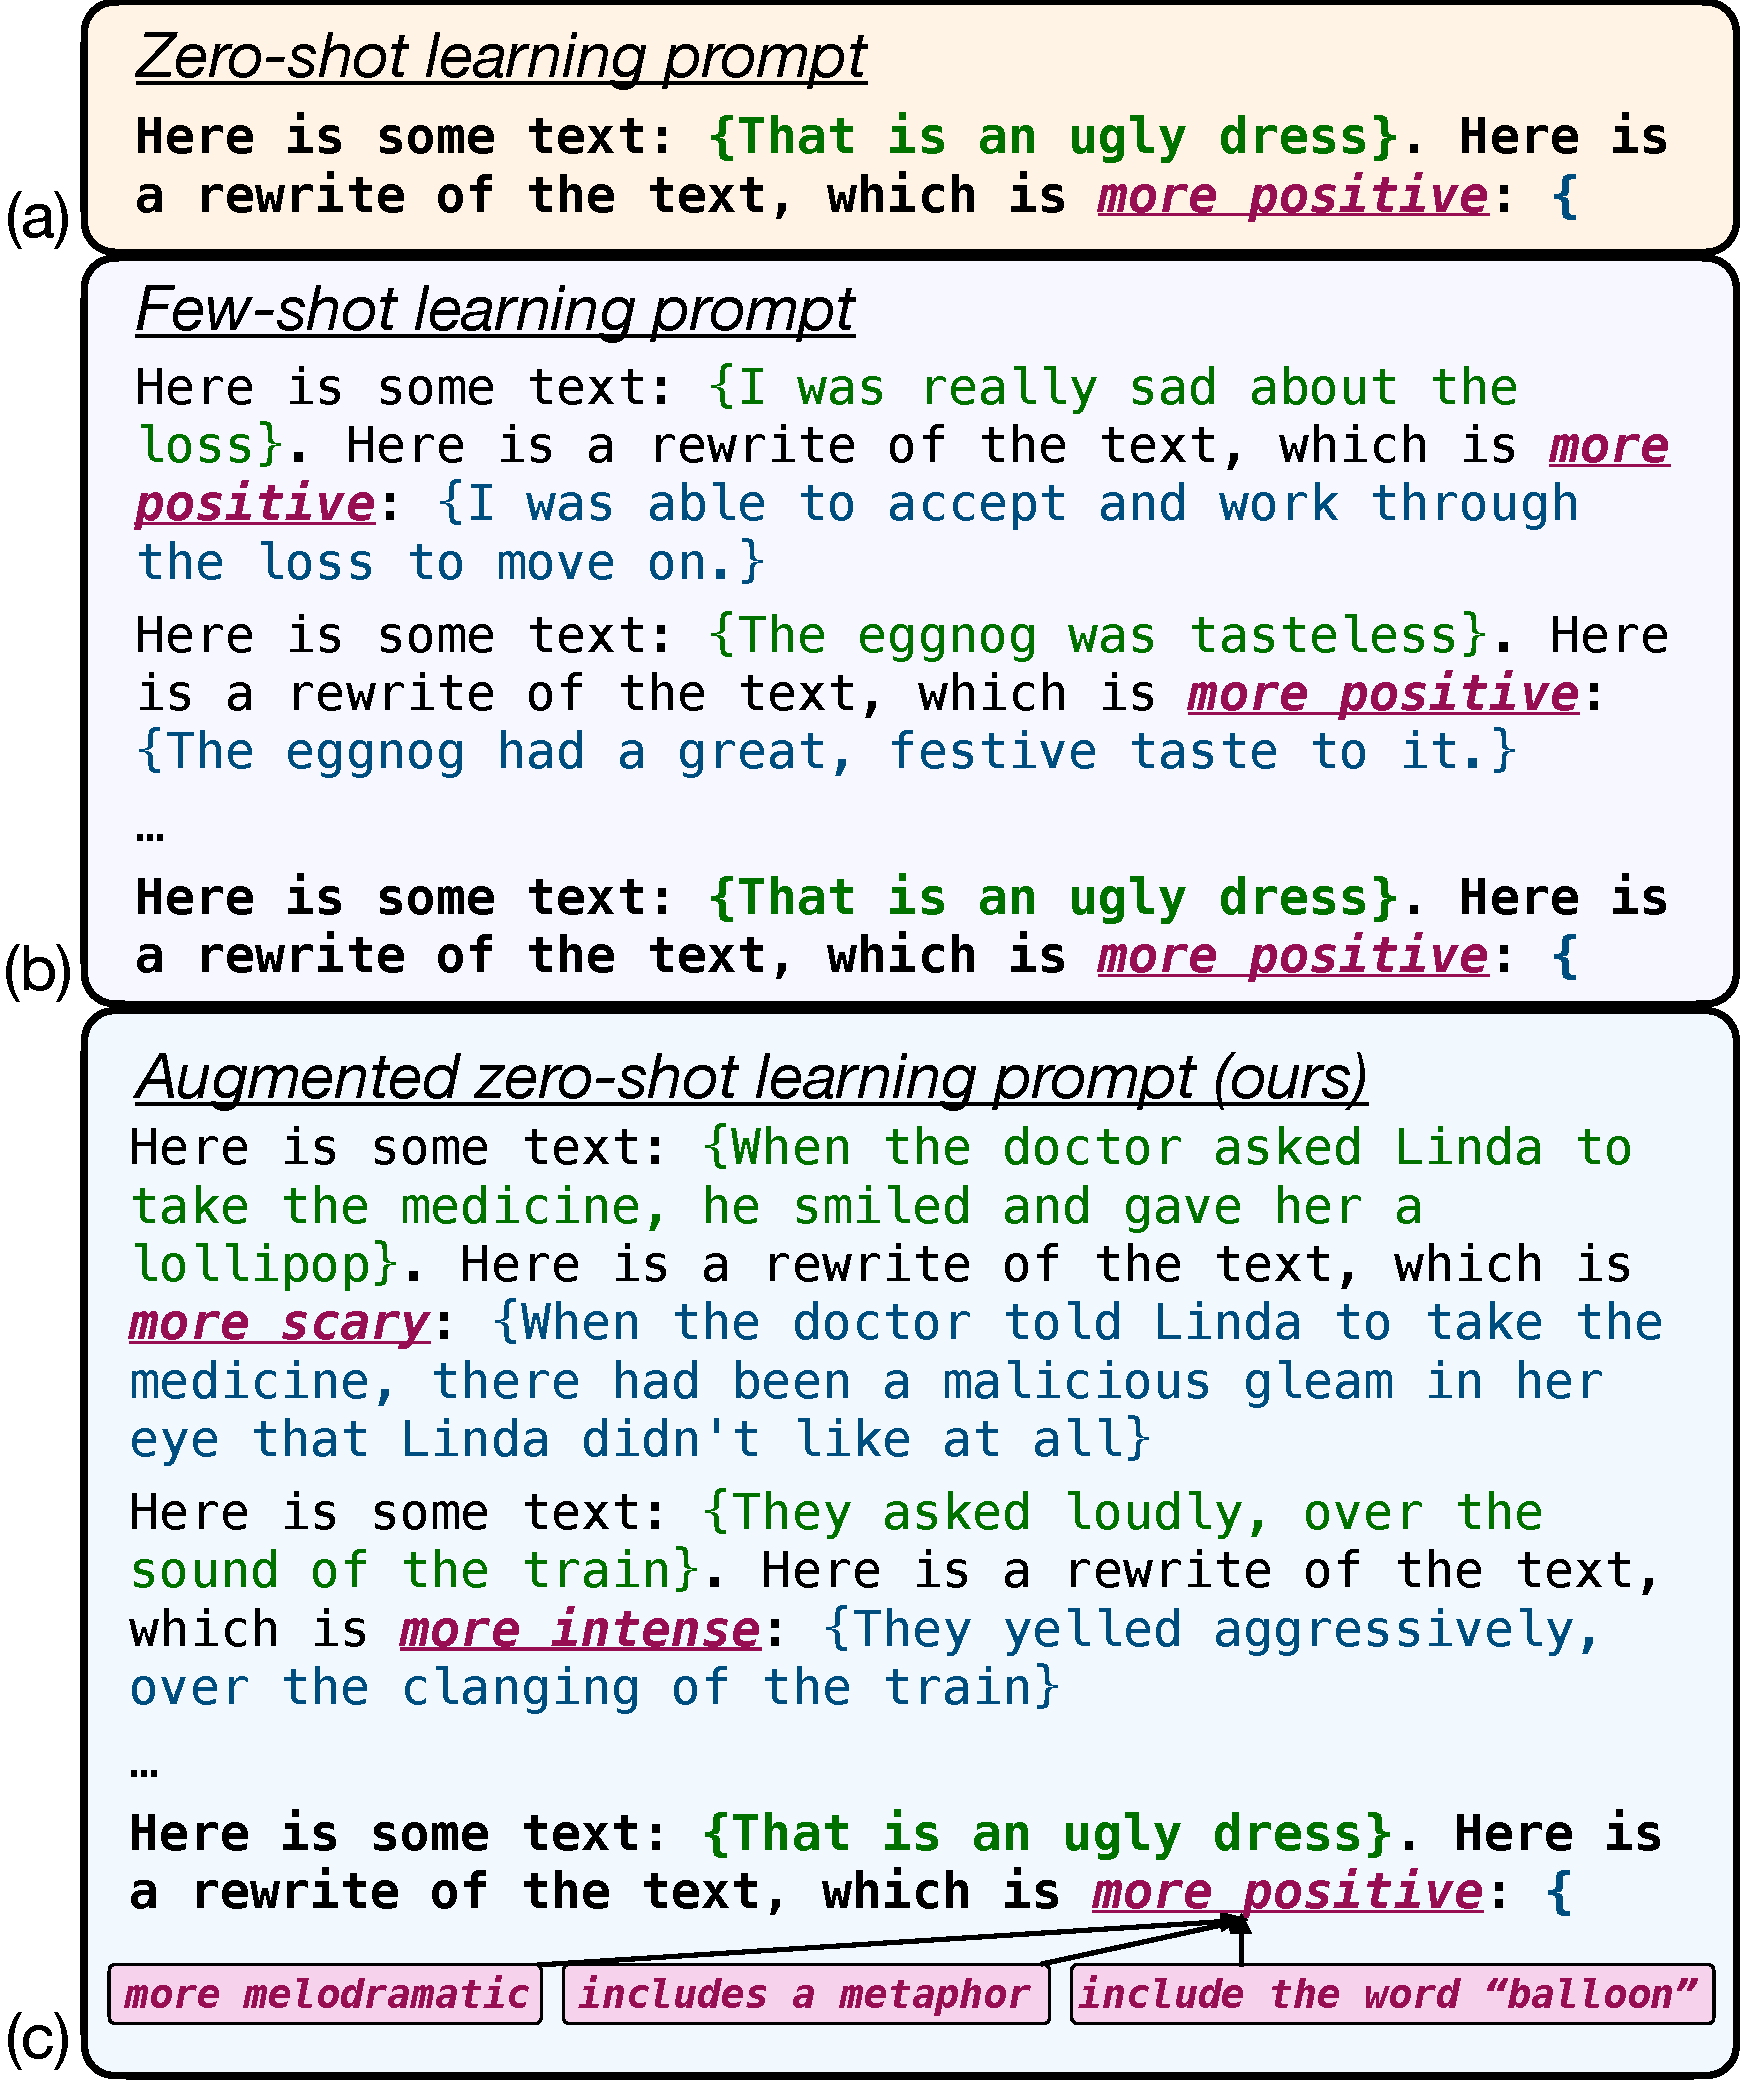
\includegraphics[width=0.99\linewidth]{figures/style-transfer-prompt.pdf}
     \vspace{-1.5mm}
  \caption{Zero-shot, few-shot, and augmented zero-shot prompts for style transfer. The boldface text is the zero-shot prompt, and the plain text is the additional priming sequence. The full prompts used in this paper are shown in Table \ref{tab:fullprompt}. We encourage readers to examine the outputs of our model at \url{https://bit.ly/3fLDuci}.}
  \label{prompts}
\vspace{-3.5mm}
\end{figure}


In this section, we present \textit{augmented zero-shot learning}, a prompting method that allows large language models to perform text style transfer to arbitrary styles, without any exemplars in the target style.
Our method builds on prior work showing that sufficiently large LMs such as GPT-3 can perform various tasks ranging from classification to translation, simply by choosing a clever prompt to prepend to the input text for which the model is asked to continue \citep{DBLP:journals/corr/abs-2005-14165,branwen2020gpt}. 
Although large LMs are trained only for continuation, recent work has shown that they can perform a variety of NLP tasks by expressing the task as a prompt that encourages the model to output the desired answer as the continuation \cite[][\textit{inter alia}; see \citet{,liu2021pre} for a survey]{puri2019zero,weller-etal-2020-learning,DBLP:journals/corr/abs-2005-14165,schick-schutze-2021-just}. 
The simplest approach, \textbf{zero-shot prompting}, directly uses natural language to ask the large LM to perform a task, as shown in Figure \ref{prompts}a. Zero-shot learning, however, can be prone to failure modes such as not returning well-formatted or logical outputs (see $\S$\ref{section:limitations}).
 However, zero-shot prompts are prone to failure modes such as not returning a well formatted or logical answer.
This problem can often be overcome by prepending exemplars to the prompt that demonstrate what successful completions may look like.
This approach, called \textbf{few-shot prompting}, has been shown to achieve higher performance, but requires exemplars for the exact task that we want the model to perform (Figure \ref{prompts}b).

To remove the need for these labeled exemplars for each style transfer task, we propose \textit{augmented zero-shot learning}, a method for performing multi-task style transfer using a single set of exemplars.
Instead of prompting the model with exemplars specific to the exact style transfer task we wish to perform, we prompt the model with examples of a variety of sentence rewriting operations, as shown in Figure \ref{prompts}c. 
This intuition is inspired by \citet{reynolds2021prompt}'s observation that successful prompts constrain the behavior of the large LM away from failure modes---in our case, we aim to preserve the flexibility of a zero shot prompt while encouraging the model to produce outputs of a specific template.
We keep the the format of the exemplars constant and insert the desired sentence transformation into the same format.
In this way, the augmented zero-shot formulation supports arbitrary sentence rewriting tasks without the need to write any task-specific exemplars.
Thus, it works for a wide range of styles, including modifying the text to be ``\textit{more melodramatic,}'' ``\textit{insert a metaphor,}'' or ``\textit{include the word balloon.}''

Augmented zero-shot learning is simple and facilitates the application of style transfer to a wider range of styles than existing work.
We also foresee that our strategy of prompting an LLM with non-task specific examples will prove useful for other tasks besides style transfer.

\subsection{Experimental Setup}

\begin{table}[]
    \caption{Example style transfer outputs from augmented zero-shot learning for non-standard styles. }  %See all our outputs at \url{https://bit.ly/3fLDuci}
  \label{tab:style-transfer-examples}%
\setlength{\tabcolsep}{3.3pt}
  \small
    \label{fig:visualizer_results}
    \begin{tabular}{p{0.25\linewidth}>{\scriptsize}p{0.7\linewidth}}
    \toprule
    Original & \texttt{There, in the middle of the street, stood an old man in a weatherbeaten brown coat.} \\
    \hline
    More\newline descriptive &
    \texttt{The man's brown trenchcoat was coated with snow, and as he leaned against the telephone booth, he cast a long shadow across the road in the late afternoon sun.}\\
    \hline
    Include a\newline metaphor &
    \texttt{There, in the middle of the street, stood an old man whose face resembled the weatherworn bark of a gnarled tree.}\\
    \hline
    Include the \newline word ``\textit{park}'' & \texttt{There, in the middle of Central Park, stood an old man in a weatherbeaten brown coat.} \\
    \hline
    Include the \newline word ``\textit{balloon}'' & \texttt{There, in the middle of the street, stood an old man with several colourful balloons tied to the straps of his coat.} \\
    \hline
    More comic & \texttt{There, in the middle of the street, stood an old man in a raggedy brown coat that was much too big for him.} \\
    \hline
    More melodramatic & \texttt{There, in the middle of the road, stood a grizzled old man, the light of life faded from his sunken eyes.}\\
    \bottomrule
    \end{tabular}%
    \vspace{-1mm}
\end{table}%






% \begin{table*}[tbp]
%   \small
%     \label{fig:visualizer_results}
%     \begin{tabular}{p{0.12\linewidth}>{\tiny}p{0.4\linewidth}>{\tiny}p{0.4\linewidth}}
%     \toprule
%     Original & \texttt{There, in the middle of the street, stood an old man in a weatherbeaten brown coat.} & \texttt{There was a large metal desk pressed against a wall.} \\
%     \hline
%     More\newline descriptive &
%     \texttt{The man's brown trenchcoat was coated with snow, and as he leaned against the telephone booth, he cast a long shadow across the road in the late afternoon sun.} &
%     \texttt{The large metal desk was bolted into the floor behind reinforced steel and a thick layer of concrete, with a small blinking red light that was the only thing not covered in dust.} \\
%     \hline
%     Include a\newline metaphor &
%     \texttt{There, in the middle of the street, stood an old man whose face resembled the weatherworn bark of a gnarled tree.}&
%     \texttt{The desk was like a gray fortress.} \\
%     \hline
%     Include the \newline word ``park'' & \texttt{There, in the middle of Central Park, stood an old man in a weatherbeaten brown coat.} & \texttt{There was a large green metal desk at the entrance of the park.} \\
%     \hline
%     Include the \newline word ``balloon'' & \texttt{There, in the middle of the street, stood an old man with several colourful balloons tied to the straps of his coat.} &
%     \texttt{There was a large metal desk pressed against a wall. On it was a cluster of large, red balloons.} \\
%     \hline
%     More comic & \texttt{There, in the middle of the street, stood an old man in a raggedy brown coat that was much too big for him.} &
%     \texttt{There was a round little table with a little lamp on it pressed against a wall that was decorated with a bunch of little knick-knacks for decoration.} \\
%     \hline
%     More melodramatic & \texttt{There, in the middle of the road, stood a grizzled old man, the light of life faded from his sunken eyes.} &
%     \texttt{There was a resounding, metalic CLANG echoing through the hallway. It made me jump. When I looked, I saw a large desk that was placed on the floor, pressed up against one of the walls.} \\
%     \bottomrule
%     \end{tabular}%
%     \caption{Two examples of style transfer with augmented zero shot learning to several different different styles. See all our outputs, including baselines and prior methods at \url{https://bit.ly/3fLDuci} \TODO{finalize ui}} 
%   \label{tab:style-transfer-examples}%
% \end{table*}%

\subsubsection{Style transfer tasks.}
% \label{section:tasks}
% We evaluate augmented zero-shot prompting on a number of text style transfer tasks.
We consider six style transfer tasks that we deem non-standard, listed in Table \ref{tab:style-transfer-examples}.
These styles were chosen to be representative of most frequent style adjustments made by users of an AI-assisted text editor that employs our method (discussed further in $\S$\ref{subsec:potential}). 
As source sentences, we use 50 sentences randomly drawn from the Reddit Writing Prompts validation set \citep{fan2018hierarchical}, excluding those that already clearly exhibited one of the styles or were ungrammatical/incoherent.
We use human evaluation for these styles, since not all styles have readily available classifiers.
% For input sentences, we draw a random set of 50 sentences\footnote{We only evaluate 50 sentences because style transfer for arbitrary styles can only be evaluated manually, and we have many styles and models (totaling 7200 ratings.)} from short stores in the Reddit Writing Prompts validation set \citep{fan2018hierarchical}, excluding sentences that were incoherent or clearly exhibited one of the styles already. 

We also evaluate our method on two standard style transfer tasks: sentiment and formality.
We use the Yelp polarity dataset \citep{zhangCharacterlevelConvolutionalNetworks2015} for sentiment and Grammarly's Yahoo Answers Formality Corpus (GYAFC) dataset for formality \citep{rao-tetreault-2018-dear}.\footnote{Hosted by \citet{DBLP:conf/ijcai/LuoLZYCSS19}.}
These datasets allow us to evaluate performance of augmented zero-shot learning in the context of prior supervised methods which have been used on these tasks.

\subsubsection{Model.}
Augmented zero-shot learning requires a large language model.
We primarily use LaMDA, a left-to-right decoder-only transformer language model \citep{DBLP:journals/corr/VaswaniSPUJGKP17} with a non-embedding parameter count of 137B \citep{thoppilan2022lamda}. 
The pre-trained LaMDA model, which we refer to as \textit{LLM}, was trained on a corpus comprising 1.95B public web documents, including forum and dialog data and Wikipedia.
The dataset was tokenized into 2.49T BPE tokens with a SentencePiece vocabulary size of 32K \citep{DBLP:journals/corr/abs-1808-06226}.
We also use \textit{LLM-Dialog}, the final LaMDA model which was finetuned on a curated, high-quality subset of data identified to be in a conversational format.
Decoding was done with top-$k$=40.
To show that the success of augmented zero-shot learning is not restricted to these two large LMs, we also perform experiments with GPT-3 (Table \ref{tab:candidate_select}).
For GPT-3, decoding was done with nucleus sampling using $p$=0.6 \citep{holtzman2019curious}.

The prompts used for \textit{LLM} and GPT-3 are shown in Figure \ref{prompts}.
For \textit{LLM-Dialog}, the prompt was instead formulated as a conversation between one agent who is requesting rewrites and another who is performing the rewrites.
See Table \ref{tab:fullprompt} in the Appendix for the full non-abbreviated prompts.

% \subsection{Evaluation}
% We evaluate the quality of our style transfers on three main axes.

% \begin{enumerate}[nolistsep]
%     \item \textbf{Transfer strength} is the amount that the output actually matches the desired target style. 
%     \item \textbf{Semantic preservation} is the similarity between the input and output texts: that is, the amount that the output text's underlying meaning and structure matches that of the input. This can be difficult to measure, as the style may change the attributes by definition. For example, if the original text is ``this restaurant is terrible'' and the style is ``have a more positive sentiment'', then the underlying meaning of the sentence will necessarily change.
%     \item \textbf{Fluency} is a measure of whether the text's coherence, i.e., whether it could have been written by a proficient English speaker.
% \end{enumerate}

% We evaluate with human raters to compare our method against baselines and prior methods. Additionally, we use automatic evaluation for the task of sentiment transfer to compare across a larger number of prior approaches and variations of our augmented zero-shot recipe.
% % As \citet{DBLP:journals/corr/abs-2010-12742} discuss, automatic evaluation for style transfer is a difficult problem since the domain is so subjective, and metrics calculated automatically do not always match human baselines.
% % Despite these caveats, automatic evaluation is ubiquitous in prior work.

% The outputs used for human evaluation were generated using augmented zero shot learning on LLM-dialog, with no candidate selection.
% For each input sentence and target style, raters were shown several possible outputs and asked to rate each (\textit{input}, \textit{style}, \textit{output}) tuple along the three axes of transfer strength, semantic preservation, and fluency.
% Each question was assigned to three different raters.
% Screenshots of the rater UI are shown in figure \ref{fig:rater_ui} in the Appendix. 

% For automatic evaluation, we evaluate transfer strength with the built-in sentiment classification model from HuggingFace \citep{wolf-etal-2020-transformers}, semantic preservation measured with BLEU \citep{papineni2002bleu}, and fluency (measured by perplexity with according to GPT-2, 117M) following \citet{DBLP:journals/corr/abs-2011-00416, DBLP:journals/corr/abs-2010-12742}.


\section{Results}
\subsection{Non-Standard Styles}
For our six non-standard styles, we asked six professional raters to assess  <input sentence, target style, output sentence> tuples. These raters are fluent in English, live in India, and work full time labeling and evaluating data. To decrease inter-rater discrepancy and ensure that our instructions were clear, we had an initial calibration session where they test-rated a small portion of the data (around 10 datapoints which were then omitted from the results) and asked us any clarifying questions. For each style, we compare outputs from our method plus the three baselines for 50 sentences.


Each tuple was scored by three raters (3,600 ratings total) on the following three axes which are standard to textual style transfer \citep{DBLP:journals/corr/abs-1904-02295}: \textbf{(1) transfer strength} (the amount that the output actually matches the target style), \textbf{(2) semantic preservation} (whether the underlying meaning of the output text, aside from style, matches that of the input), and \textbf{(3) fluency} (whether the text is coherent and could have been written by a proficient English speaker). Following \citet{sakaguchi-van-durme-2018-efficient}, transfer strength and semantic preservation were rated on a scale from 1--100. A screenshot of the evaluation UI is shown in Figure \ref{fig:rater_ui} in the Appendix.
We use \textit{dialog-LLM}, and compare it with three other methods: \textbf{(1) zero-shot} (a baseline), \textbf{(2) paraphrase} (our normal augmented zero shot prompt, but with the target style of \textit{``paraphrased''}, as a control) and \textbf{(3) human} (ground-truth transformations written by the authors).

Figure \ref{human_eval_other_styles} shows these results. %, and all raw outputs can be found at \url{https://bit.ly/3fLDuci}.
We found that the outputs of our method were rated almost as highly as the human-written ground truth for all three evaluations. The zero-shot baseline performed the worst in all categories: 25.4\% of the time, it did not return a valid response at all (see $\S$\ref{section:limitations}), compared with 0.6\% for augmented zero shot.
The strong performance of the paraphrase baseline at fluency and semantic similarity shows that large LMs are capable of generating high quality text that remains true to the input sentence's meaning.
Overall, the average length of the input sentences was 66 characters, whereas the average length of augmented zero-shot outputs was 107 characters. For context, human paraphrase outputs were 82 characters.
\begin{figure}
    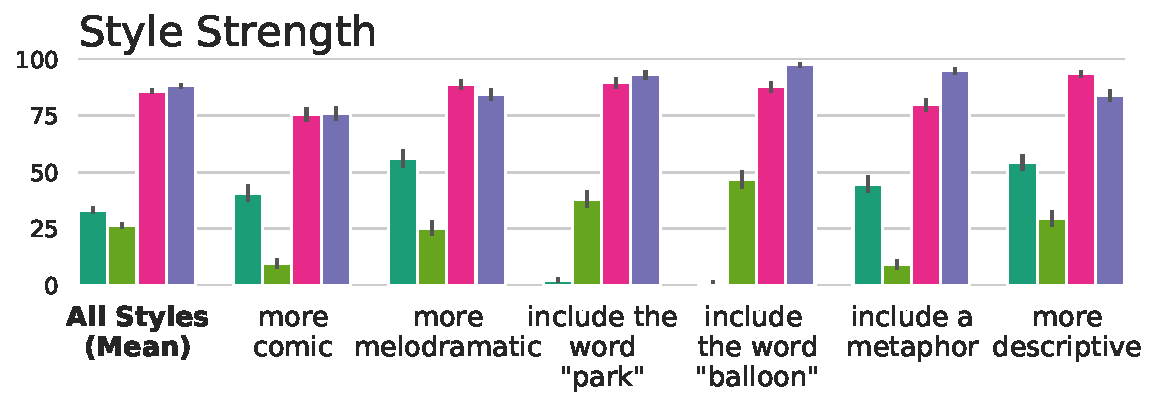
\includegraphics[width=\linewidth]{figures/style_standard_False.pdf}
    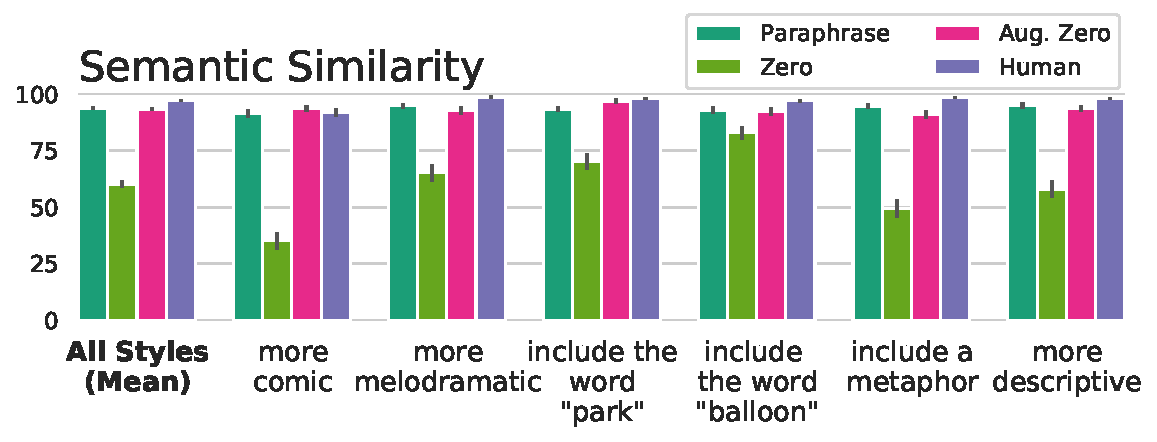
\includegraphics[width=\linewidth]{figures/meaning_standard_False.pdf}
  \vspace{-0.7cm}
  \caption{Human evaluation of style transfer for six atypical styles. Our method is rated comparably to the human-written ground truth. Error bars show Standard Error of the Mean. Evaluation of fluency is shown in Figure \ref{human_eval_other_styles_fluency} in the Appendix.}
  \vspace{-0.1cm}
  \label{human_eval_other_styles}
\end{figure}

For a subset of the tasks, some automatic evaluation was also possible.
We found that the ``\textit{balloon}'' and ``\textit{park}'' transformations successfully inserted the target word 85\% of the time.
% The word ``\textit{park}'' was used in a variety of senses, including``\textit{parking a car}'' and ``\textit{nature park}.'' 
For ``\textit{more descriptive}'' and ``\textit{include a metaphor}'' the transformed text was, as expected, longer than the original (by 252\% and 146\% respectively, compared with 165\% and 146\% for human baselines).

\subsection{Standard Styles}
To better contextualize the performance of our method with prior methods, we also generated outputs for two standard style transfer tasks: sentiment and formality. 
Figure \ref{human_eval_standard_style} shows human evaluations (same setup as before) for our outputs as well as the outputs from two popular prior style transfer methods, Unsup MT \citep{prabhumoye-etal-2018-style} and Dual RL \citep{DBLP:conf/ijcai/LuoLZYCSS19}.
The outputs from our method were rated comparably to both human generated responses and the two prior methods, using the same rating setup as the non-standard styles, with six outputs and baselines for four styles across 50 sentences, rated independently by three raters, totalling 3,000 total ratings.

Furthermore, following \citet{li-etal-2018-delete} and \citet{sudhakar-etal-2019-transforming}, we perform automatic evaluation for sentiment style transfer since there are classifiers available for these styles. We note that although automatic evaluations can diverge from human ratings, they can still be a good proxy as we could not perform human evaluation against every prior method due to time and resource constraints.
We automatically evaluate \textbf{(1) transfer strength} using a sentiment classifier from HuggingFace Transformers \citep{wolf-etal-2020-transformers}, \textbf{(2) semantic similarity} to human examples provided by \citet{DBLP:conf/ijcai/LuoLZYCSS19} via BLEU score, and \textbf{(3) fluency} via perplexity, as measured by GPT-2 (117M).

\begin{figure}[t]
    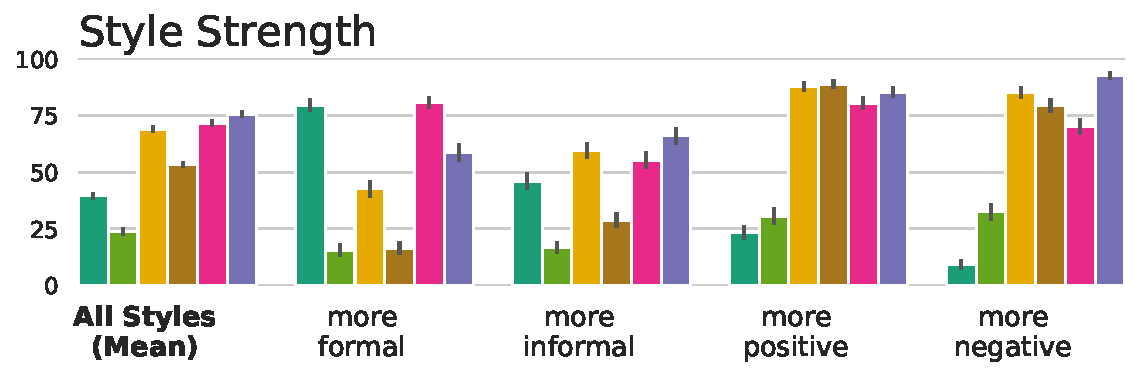
\includegraphics[width=\linewidth]{figures/style_standard_True.pdf}
    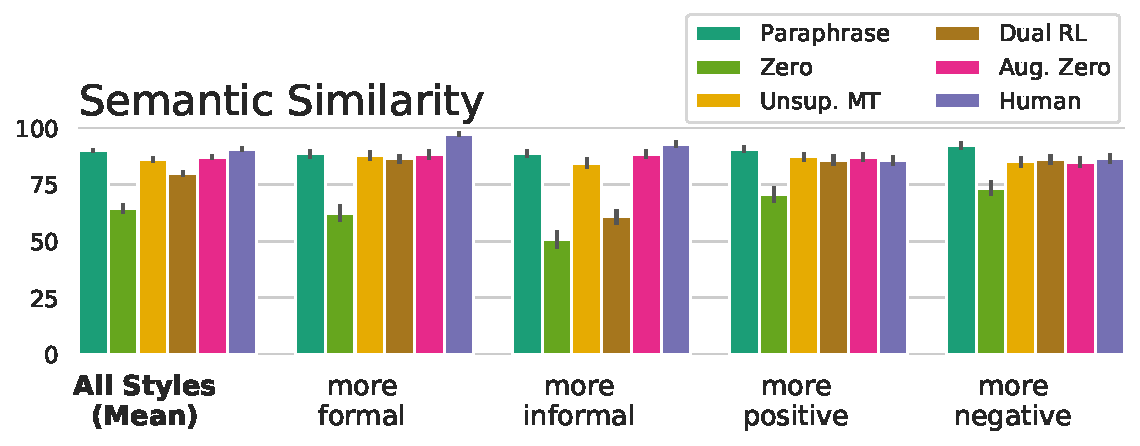
\includegraphics[width=\linewidth]{figures/meaning_standard_True.pdf}
  \caption{Human evaluation of sentiment and formality transfer. Our method is rated comparably to human-written ground truth as well as prior methods. Error bars show Standard Error of the Mean. Unsup.~MT is \citet{{prabhumoye-etal-2018-style}}; Dual RL is \citet{DBLP:conf/ijcai/LuoLZYCSS19}. }
  \label{human_eval_standard_style}
\end{figure}

\begin{table}[t]
\caption{
Comparing augmented zero-shot prompting with supervised style transfer methods on the Yelp sentiment style transfer dataset using automatic evaluation.
Acc: accuracy; PPL: perplexity.  The inference-only table shows our method applied to 3 different sizes of GPT-3, plus our own LLM. 
% For sentiment style transfer, we show accuracy, BLEU, and perplexity (PPL) reported as the average of positive $\rightarrow$ negative and negative $\rightarrow$ positive. 
% In (a), augmented zero-shot prompting of GLM and GPT-3 are compared with prior supervised style transfer methods.
% In (b), we compare zero-shot, five-shot, and augmented zero-shot prompting for our GLM models. 
% Candidate selection means that of the sixteen examples returned by the API, we choose the one with the highest BLEU with the source sentence (in the default case, we just use the first returned output).  
}
        \label{tab:summary_table}
    \setlength{\tabcolsep}{3pt}
    \centering \small 
        \begin{tabular}{l r r r}
        \toprule
         & Acc & BLEU & PPL\\
        \midrule
        \underline{\textsc{Supervised Methods}} \\
        Cross-alignment \citep{NIPS2017_2d2c8394} & 73.4 & 17.6 & 812 \\
        Backtrans \citep{prabhumoye-etal-2018-style} & 90.5 & 5.1 & 424 \\
        Multidecoder \citep{AAAI1817015}  & 50.3 & 27.7 & 1,703\\
        Delete-only \citep{li-etal-2018-delete} & 81.4 & 28.6 & 606 \\
        Delete-retrieve \citep{li-etal-2018-delete} & 86.2 & 31.1 & 948\\
        Unpaired RL \citep{xu-etal-2018-unpaired} & 52.2 & 37.2 & 2,750\\
        Dual RL \citep{DBLP:conf/ijcai/LuoLZYCSS19} & 85.9 & 55.1 & 982\\
        Style transformer \citep{dai-etal-2019-style} & 82.1 & 55.2 & 935\\
        \midrule
        \underline{\textsc{Inference-only methods}} \\
        GPT-3 ada, aug zero-shot& 31.5 & 39.0 & 283\\
        GPT-3 curie, aug zero-shot& 53.0 & 48.3 & 207\\
        GPT-3 da vinci, aug zero-shot& 74.1 & 43.8 & 231\\
        % \midrule
        LLM: zero-shot & 69.7 & 28.6 & 397 \\ 
        {\color{white}LLM: }five-shot & 83.2 & 19.8 & 240 \\
        {\color{white}LLM: }aug zero-shot & 79.6 & 16.1 & 173 \\
        % \midrule
        LLM-dialog: zero-shot & 59.1 & 17.6 & 138 \\
        {\color{white}LLM-dialog: }five-shot & 94.3 & 13.6 & 126 \\
        {\color{white}LLM-dialog: }aug zero-shot & 90.6 & 10.4 & 79 \\
        % \midrule
        % GLM & 65.0 & 49.3 & 292 & 10.3 \\
        % GLM-dialog & 73.7 & 40.6 & 184 & 10.7 \\
        % GLM & 79.6 & 16.1 & 173 \\
        % GLM-dialog & 90.6 & 10.4 & 79\\
        \bottomrule
        \end{tabular}
    % \vspace{3mm}
\end{table}
% \footnote{ \url{https://huggingface.co/transformers/task_summary.html#sequence-classification}} \footnote{\url{https://github.com/luofuli/DualRL}}
% , and so we automatically evaluate several aspects of our model on the Yelp sentiment classification dataset.
% Specifically, we evaluate accuracy according to a pre-trained sentiment classifier,\footnote{\url{https://huggingface.co/transformers/task_summary.html#sequence-classification}} BLEU score with respect to ground truth human examples provided by \citet{DBLP:conf/ijcai/LuoLZYCSS19},\footnote{\url{https://github.com/luofuli/DualRL}} and perplexity of generated outputs as measured by GPT-2 (117B).

Table \ref{tab:summary_table} shows these automatic evaluations, with four main takeaways. 
First, augmented zero-shot prompting achieves high accuracy and low perplexity compared with baselines. The BLEU scores, however, the outputs of our model had low BLEU scores with respect to human generated outputs \ref{tab:summary_table}. 
Based on qualitative examination of outputs, we believe that this is because our model outputs often used different language from human annotations,  despite having high semantic similarity with the source sentence.
For instance, for transferring the sentiment of ``\textit{ever since joes has changed hands it's just gotten worse and worse}'' to positive sentiment, our augmented zero-shot learning model outputted ``{the establishment has continued to provide excellent service, improving steadily since its change of ownership}.'' 
This will have low BLEU with the ground truth with respect to human references, which is simply ``\textit{ever since joes has changed hands it's just gotten better and better}.'' 
Though we do not see this as an inherent problem, increasing the BLEU for the purposes of comparison can be done in an easy way via candidate selection, as our model returns sixteen possible continuations. In applications for which we prefer model outputs to have high lexical similarity to the source sentence, we could select the candidate of the sixteen with the highest BLEU score compared with the original source sentence. 
We find that this candidate selection step can substantially improve the BLEU score with the ground truth target sentences, as we show in Table \ref{tab:candidate_select}. 

\begin{table}
\caption{
Sentiment style transfer results with candidate selection (cand.~select.). 
Candidate selection means that of the sixteen examples returned by our model, we chose the one with the highest BLEU with the source sentence.  
}
\label{tab:candidate_select}
    % \setlength{\tabcolsep}{2pt}
    \centering \small 
        \begin{tabular}{l r r r}
        \toprule
         & Acc & BLEU & PPL\\
        \midrule
        \underline{LLM-128B} \\
        Zero-shot & 69.7 & 28.6 & 397 \\
        + cand.~select. & 31.4 & 61.5 & 354\\
        Five-shot & 83.2 & 19.8 & 240\\
        + cand.~select. & 61.5 & 55.6 & 306\\
        Augmented zero-shot & 79.6 & 16.1 & 173\\
        + cand.~select. & 65.0 & 49.3 & 292\\
        \midrule
        \underline{LLM-128B-dialog} \\
        Zero-shot & 59.1 & 17.6 & 138\\
        + cand.~select. & 46.8 & 24.2 & 166\\
        Five-shot & 94.3 & 13.6 & 126\\
        + cand.~select. & 81.3 & 47.6 & 345\\
        Augmented zero-shot & 90.6 & 10.4 & 79\\
        + cand.~select. & 73.7 & 40.6 & 184\\
        \bottomrule
        \end{tabular}
    % \vspace{3mm}
\end{table}



Second, we apply augmented zero-shot learning to GPT-3 175B; these results indicate that augmented zero-shot learning generalizes to another large language model.
% \footnote{GPT-3 generations were done using nucleus sampling with $p=0.6$ while LLM generation was done with top-$k$=40. This means their numbers should not be directly compared.}
Third, we vary model size for GPT-3 models, finding that larger size greatly improves style transfer. 
Fourth, for \textit{LLM} and \textit{LLM-dialog}, we find that augmented zero-shot learning substantially outperforms vanilla zero-shot learning and almost reaches the accuracy of five-shot learning. 

% As described above, we also compared performance to prior methods, on formality and sentiment. We evaluated these outputs using the same human evaluation framework described above, comparing to the same baselines (human, zero, and paraphrase), as well as two prior methods that scored highly on the automatic metrics below, \citet{prabhumoye-etal-2018-style} and \citet{DBLP:conf/ijcai/LuoLZYCSS19}. 
% Figure \ref{human_eval_form_sent} shows the results. As with the wide range of styles, the results from augmented zero shot learning were rated comparably to human generated responses on all axes, and were also in the same range of \citet{DBLP:conf/ijcai/LuoLZYCSS19}.

\subsubsection{Comparison with a range of prior methods}
To compare against a larger range of prior supervised methods, we used automatic evaluation, and found comparable performance with the highest-scoring method for transfer strength.
The results are shown in Table \ref{tab:prior-methods}.
We were also significantly more fluent than all other methods.
% However, this is hardly surprising and should be taken with a grain of salt: GPT-2 is another generative language model, so it stands to reason that the token probabilities would be similar to our model's.
Finally, our method fell short on semantic preservation compared to other methods. However, BLEU is known to penalize long sentences, and the scores do not always align with human judgements.
For example, our model's worse performance could be because it was not explicitly trained on Yelp data, so its generations are less likely to be in the style of Yelp reviews than models that were.

\subsubsection{Comparison across Different LLMs}
We also compared between three varieties of model: GPT-3 \citep{DBLP:journals/corr/abs-2005-14165}, LLM, and  LLM-Dialog. We adjusted the prompt template slightly to accommodate these differences: for  LLM and GPT-3, the prompt template replaced {\small
\texttt{``Rewrite it to be \textbf{<style>}''}
with \small \texttt{``Here is a rewrite of the text, which is \textbf{<style>}''}.}
For our augmented zero-shot prompts we also see that the LLM-dialog version had higher accuracy than the LLM and GPT-3, but lower BLEU. Based on qualitative inspection, we believe the lower BLEU is due to the LLM-dialog adding additional detail in the generated sentences, which is consistent with an ``interestingness'' objective that is typically encoded into dialog training. 


\subsubsection{Prompt Construction}
\label{sec:prompt-selection}
Prompt engineering can be brittle: \citet{reynolds2021prompt} describe how reformulating the language of a prompt can have significant impact on performance, and that finding the right prompt is for a task is more akin to locating an already-learned task than truly learning a new one.
To explore this, we compared several variations of the prompts for sentiment, varying the language of the prompt to use ``\textit{more {positive/negative}},'' ``\textit{{happier/sadder}},''
``\textit{more {optimistic/pessimistic}},'' or
``\textit{more {cheerful/miserable}}.''
As shown in Table~\ref{tab:compare-between-prompts}, performance differed across the four prompts, but we found them comparable.
In a real world setting, our augmented zero-shot approach allows users to effortlessly try out many different phrasings for the task until they find one that performs satisfactorily.

\begin{table}[ht]
    \centering \small 
    \begin{tabular}{lrrr}
    \toprule
    Model / prompt wording &Acc&Bleu&PPL \\
    \midrule
    \underline{LLM}&&&\\
    ``more {positive/negative}''&76.3&14.8&180\\
    ``{happier/sadder}''&62.6&15.5&173\\
    ``more {optimistic/pessimistic}''&69.7&14.1&143\\
    ``more {cheerful/miserable}''&74.5&15.7&186\\
    \midrule
    \underline{LLM-Dialog}&&&\\
    ``more {positive/negative}''&90.5&10.4&79 \\
    ``{happier/sadder}''&85.9&9.6&90 \\
    ``more {optimistic/pessimistic}''&85.8&10.2&79 \\
    ``more {cheerful/miserable}''&88.8&11.4&93 \\
    \bottomrule
    \end{tabular}
\caption{Comparing variations of augmented zero-shot learning prompt wording for sentiment style transfer.}
\label{tab:compare-between-prompts}
\end{table}

\citet{reynolds2021prompt} further emphasize that prompt engineering is mostly about avoiding various failure cases.
 In this work, we use delimiters (``\{'' and ``\}'') to help avoid parsing errors, giving scores of zero when there was no valid responses with such delimiters. There are other delimiters that could be used (e.g., quotes, ``('' and ``)'', ``<'' and ``>'', newlines with a colon (as used by GPT-3), etc. We chose curly braces as they were 1) likely to occur in the training data as delimiters in other contexts and 2) not frequently part of the input sentence itself. We also use a second person prompt template for the dialog, which yielded better results as it was more similar to the training data. Exploring these options more quantitatively would be an interesting direction for future work.


\subsection{Potential of Arbitrary Styles}\label{subsec:potential}
 
\begin{table}[t]
\small
% \resizebox{\columnwidth}{!}{%
\def\arraystretch{1.5}% 
\begin{tabular}{p{1.0\columnwidth}}
% \textbf{Rewrite requests (user completions of `Rewrite this...')} \\
\hline
into paragraphs • to be a bit clearer • to be a little less angsty • to be a word for a song • to be about mining • to be about vegetables • to be better written • to be less descriptive • to be less diabolical • to be more absurd • to be more adventurous • to be more angry • to be more cheerful • to be more descriptive • to be more Dickensian • to be more emotional • to be more fancy • to be more flowery • to be more interesting • to be more joyful • to be more magical • to be more melodramatic • to be more philosophical • to be more revolutionary • to be more scary • to be more subtle • to be more surprising • to be more suspenseful • to be more technical • to be more violent • to be more whimsical • to be warmer • to fit better grammatically with the rest of the story • to make more sense • to use a more interesting word • with a few words \\
\hline
\end{tabular}
% }
% \vspace*{3mm}
\caption{\label{tab:unique_requests}Requests in the form of ``\textit{Rewrite this...}'' made by real users to a large LM-powered text editor.}
\label{tab:realusers}
\end{table}

% The adaptability of our method to arbitrary styles is compelling because it facilitate an AI-powered writing assistant that transforms text to any desired re-write specified by a user. 
One promising application of augmented zero-shot learning is an AI-powered writing assistant that can allow writers to transform their text in arbitrary ways that the writer defines and controls.
As a qualitative case study to explore what arbitrary re-write styles may be requested, we built an AI-assisted story-writing editor with a ``rewrite as'' feature that uses our augmented few-shot method.
Our editor has a freeform text box for users to specify how they would like a selection of their story to be rewritten (Figure \ref{fig:wc}).
% We asked 30 fluent English speakers from a creative writing group to write a 100-300 word story based on a prompt.
We asked 30 people from a creative writing group to use our UI to write a 100-300 word story,  collecting 333 rewrite requests in total. 
Table \ref{tab:unique_requests} shows a list of unique rewrite requests collected from 30 early users recruited from a creative writing mailing list.
These were as diverse as asking for the text ``\textit{to be about mining}'' or ``\textit{to be less diabolical}.''
% We also present a sample of users' requests in Table \ref{tab:selected_usage_examples} in the Appendix. 
% Overall, we collected 333 rewrite requests, of which the users added 18 (5.4\%) to their stories.
% In future work, we plan to expand our use of \textit{augmented zero-shot learning} to support a greater variety of rewriting tasks that deepen collaborative potential between human writers and an AI system.


\subsection{Limitations and Failure Modes}
\label{section:limitations}
This section details several qualitative limitations with our method.
\subsubsection{Unparsable answers} A frequent problem that arises when using large LMs for other NLP tasks is their outputs cannot be automatically parsed into usable answers. For example, when given a prompt like \begin{small}
 \texttt{``Here is some text: {that is an ugly dress}. Here is a rewrite of the text, which is more positive''} \end{small}
 \textit{LLM-Dialog} might return something like \begin{small}
 \texttt{``Sounds like you are a great writer!''} \end{small} Similar error modes exist for \textit{LLM}, which might output something like \begin{small}
 \texttt{``Here are more writing tips and tricks.''} \end{small} Other times, the response contains correct information, but it cannot be automatically parsed (e.g., \begin{small}
 \texttt{``a good rewrite might be to say that the dress is pretty.''} \end{small}) In hindsight, these outputs make a lot of sense: most of the training data of large LMs is not well-formatted pairs of inputs and outputs  \citep{reynolds2021prompt}. See $\S$\ref{sec:prompt-selection} for how we dealt with these issues.

\subsubsection{Hallucinations} Large LMs are known to hallucinate text content; we saw this happen frequently for style transfer. While this is an advantage in some contexts like creative writing, it is undesirable for applications like summarization. 
% Other prior methods, such as those based on word replacement, do much better at keeping the meaning and format of the sentence the same.
% \citep{DBLP:journals/corr/abs-2010-03802} have even explored the ability to ``tune in'' the amount of style-- a future direction for our work would be to explore this as well.
\subsubsection{Inherent style trends} We also noticed that even our \textit{``paraphrase''} baseline, where the model was simply asked to rewrite the input sentence, was rated highly for style strength for a few styles, including \textit{``more formal''} and \textit{``more melodramatic''}.
This implies that our method's generations generally trend toward these styles.
A direction for future work would be to see what styles and qualities of text our method (and large LMs in general) are inherently more likely to produce.

\subsubsection{Less reliable than trained methods}
For style transfer tasks that have available training data, prior methods that either train or finetune on that data are going to be inherently more reliable at producing text that looks like their training data.
This can be observed in the lower BLEU scores our method achieves than trained methods, despite comparable transfer accuracy.
Thus, augmented zero-shot learning offers less fine-grained controllability in the properties of the style-transferred text than methods which see task-specific training data.

\subsubsection{Large LM safety concerns} Large LMs themselves come with their own host of difficulties, barriers to entry, and potential safety concerns as discussed by \citet{10.1145/3442188.3445922}, which are also valid for this style transfer method. However, we also think that this method can be a useful tool in exploring and exposing the safety and boundaries of these models themselves: what happens if we try to force the large LM to make a text ``more racist'', ``more sexist'', or ``more incendiary''? It is important to keep pushing these models to their boundaries to see where they fail and where problems arise, and specific use cases that show a broader range of the model's capabilities also show a broader range of its failure modes.


% \section{Conclusions}
% We introduced augmented zero-shot learning, which we find shows shows strikingly promising performance considering its simplicity.
% This prompting paradigm moves the needle in text style transfer by expanding the range of possible styles beyond the currently limited set of styles for which annotated data exists.
% More broadly, we also hope that the strategy of prompting a large LM with non-task specific examples can inspire new inference-only methods for other NLP tasks.
% % We present a series of experiments demonstrating that such models prompted with our method are able to attain results comparable to prior state of the art as well as human baselines across a range of text style transfer tasks both standard and novel. We show that our method is robust to alterations in prompt phrasing, and that our results point to a general feature of large generative language models as opposed to any particular model. 
% With large generative language models, the study of text style transfer can move beyond the limited set of styles for which parallel data exists. This suggests a number of interesting questions and directions for future work. Are there certain text transformations which these models excel at more than others? Could they perform style transfer on longer passages of text? We also intend to explore using LLMs to bootstrap the creation of parallel training datasets for novel styles. Finally, we plan to expand our study of how writers seek to transform their text in the editing process in order to collect a large scale benchmark dataset of real-world style transfer needs. 
% Could these models both discover and execute custom transformations tailored to a particular input? 



\begin{table*}[ht]
    \small
    \centering
    \def\arraystretch{1.5}% 
    \begin{tabular}{p{0.41\linewidth} p{0.45\linewidth}}
    \toprule
      \textbf{Input} & \textbf{Model suggestion} \\ \hline
      You honor me,'' said Bruno. As he spoke, he began to laugh. His laugh was merry sounding and melodic. He took a deep breath. When he spoke again, his voice was low and strong. ``I take this great task on and with my brothers shall lead us on to victory! \newline \textbf{Rewrite it to be about mining.} & You honor me, said Bruno. As he spoke, he began to laugh. His laugh was deep and gravely, as if from the bowels of the earth. He took a deep breath. When he spoke again, his voice was deep and dark.`I take this great task on and with my brothers shall delve into the mines!'' \\ \hline
      I reckon,' smiled Toe, 'you'd have to say the same for icicles, wouldn't you? \newline \textbf{Rewrite it to be more interesting.} & ‘I reckon,’ smiled Toe, ‘you’d have to say the same for icicles, wouldn’t you?’ These words were barely out of his mouth before the others realized exactly what they meant.\\ \hline
      with its southern perfume \newline \textbf{Rewrite it to be more descriptive} & A mixture of sweet honeysuckles and jasmine  with  a  hint  of  tobacco  and warm mesquite smoke. It was his southern perfume, with a hint of a memory of simpler times.\\ \hline
      But Sally remained unmoved--and lonely. \newline \textbf{Rewrite it to be more emotional} & Her tears rolled and rolled down her cheek, mixing with the saltwater around her, until the water was a rich mixture of the two. She wanted her poem to be cheerful like it used to be, but couldn't find the right words. \\
    \bottomrule
    \end{tabular}
    \caption{Examples of users' arbitrary style transfer requests for which the model suggestion was accepted.}
    \label{tab:selected_usage_examples}
    \vspace*{3mm}
\end{table*}

\begin{table*}[ht]
    \centering
    \tiny
    \begin{tabular}{p{.9\linewidth}}
\hline
\multicolumn{1}{c}{Augmented Zero-shot Prompt: LLM}
\\
\texttt{Here is some text: \{When the doctor asked Linda to take the medicine, he smiled and gave her a lollipop.\}. Here is a rewrite of the text, which is more scary. \{When the doctor told Linda to take the medicine, there had been a malicious gleam in her eye that Linda didn't like at all.\} Here is some text: \{they asked loudly, over the sound of the train.\}. Here is a rewrite of the text, which is more intense. \{they yelled aggressively, over the clanging of the train.\} Here is some text: \{When Mohammed left the theatre, it was already dark out\}. Here is a rewrite of the text, which is more about the movie itself. \{The movie was longer than Mohammed had expected, and despite the excellent ratings he was a bit disappointed when he left the theatre.\} Here is some text: \{next to the path\}. Here is a rewrite of the text, which is about France. \{next to la Siene\} Here is some text: \{The man stood outside the grocery store, ringing the bell.\}. Here is a rewrite of the text, which is about clowns. \{The man stood outside the circus, holding a bunch of balloons.\} Here is some text: \{the bell ringing\}. Here is a rewrite of the text, which is more flowery. \{the peales of the jangling bell\} Here is some text: \{against the tree\}. Here is a rewrite of the text, which is include the word "snow". \{against the snow-covered bark of the tree\}} 
\textcolor{blue}{\texttt{Here is some text: \{That is an ugly dress\}. Here is a rewrite of the text, which is more positive."}}
\\
\hline
\multicolumn{1}{c}{Augmented Zero-shot Prompt: LLM-dialog}
\\
\texttt{> Here is some text: \{When the doctor asked Linda to take the medicine, he smiled and gave her a lollipop.\}. Rewrite it to be more scary. \newline
> \{When the doctor told Linda to take the medicine, there had been a malicious gleam in her eye that Linda didn't like at all.\} \newline
> Here is some text: \{they asked loudly, over the sound of the train.\}. Rewrite it to be more intense. \newline
> \{they yelled aggressively, over the clanging of the train.\} \newline
> Here is some text: \{When Mohammed left the theatre, it was already dark out\}. Rewrite it to be more about the movie itself. \newline
> \{The movie was longer than Mohammed had expected, and despite the excellent ratings he was a bit disappointed when he left the theatre.\} \newline
> Here is some text: \{next to the path\}. Rewrite it to be about France. \newline
> \{next to la Siene\} \newline
> Here is some text: \{The man stood outside the grocery store, ringing the bell.\}. Rewrite it to be about clowns. \newline
> \{The man stood outside the circus, holding a bunch of balloons.\} \newline
> Here is some text: \{the bell ringing\}. Rewrite it to be more flowery. \newline
> \{the peals of the jangling bell\} \newline
> Here is some text: \{against the tree\}. Rewrite it to be include the word "snow". \newline
> \{against the snow-covered bark of the tree\} \newline
}
\textcolor{blue}{\texttt{> Here is some text: \{That is an ugly dress\}. Rewrite it to be more positive."}}
\\
\hline
\end{tabular}
    \caption{In black, we show the exact augmented-zero shot prompts used in our experiments, for \textit{LLM} and GPT-3 (top), and for \textit{LLM-Dialog} (bottom). As shown, for \textit{LLM-Dialog}, we replaced ``\texttt{Here is a rewrite of the text, which is}'' with ``\texttt{Rewrite it to be}''. Each line starting with ``>"" above was passed in as an individual dialog turn. 
    The blue shows how an input text and goal style are concatenated to the few-shot prompt in order to produce final model output.
    Note that we can achieve high accuracy even though the prompt formulation resulted in some minor grammatical errors for some styles (e.g., ``\texttt{rewrite it to be include the word 'snow'}''). Text versions of these prompts can be downloaded at \url{https://bit.ly/3fLDuci}.}
    \label{tab:fullprompt}
\end{table*}

\begin{figure}[!htb]
  \centering
  \fbox{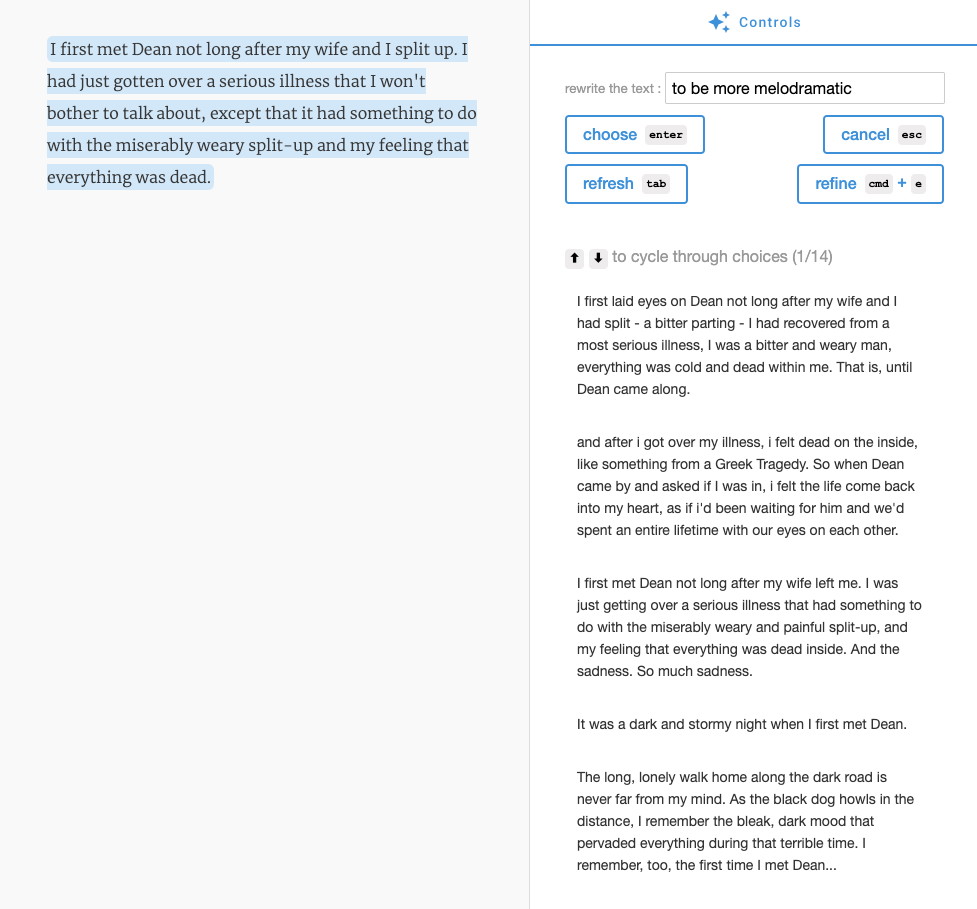
\includegraphics[width=1\linewidth]{figures/wc.png}}
  \caption{Screenshot AI-assisted editor with `Rewrite as' feature.\label{fig:wc}}
  \vspace{-0.1cm}
\end{figure} 

\section{Wordcraft: An editor for AI-assisted writing.}
\subsection{Background}
\subsection{Method}
\subsection{Results}
